\documentclass[border=12pt]{standalone}
\usepackage{tikz}
\usetikzlibrary{arrows.meta, positioning, calc, fit, backgrounds, matrix}
\usepackage{amsmath, amssymb}

\begin{document}
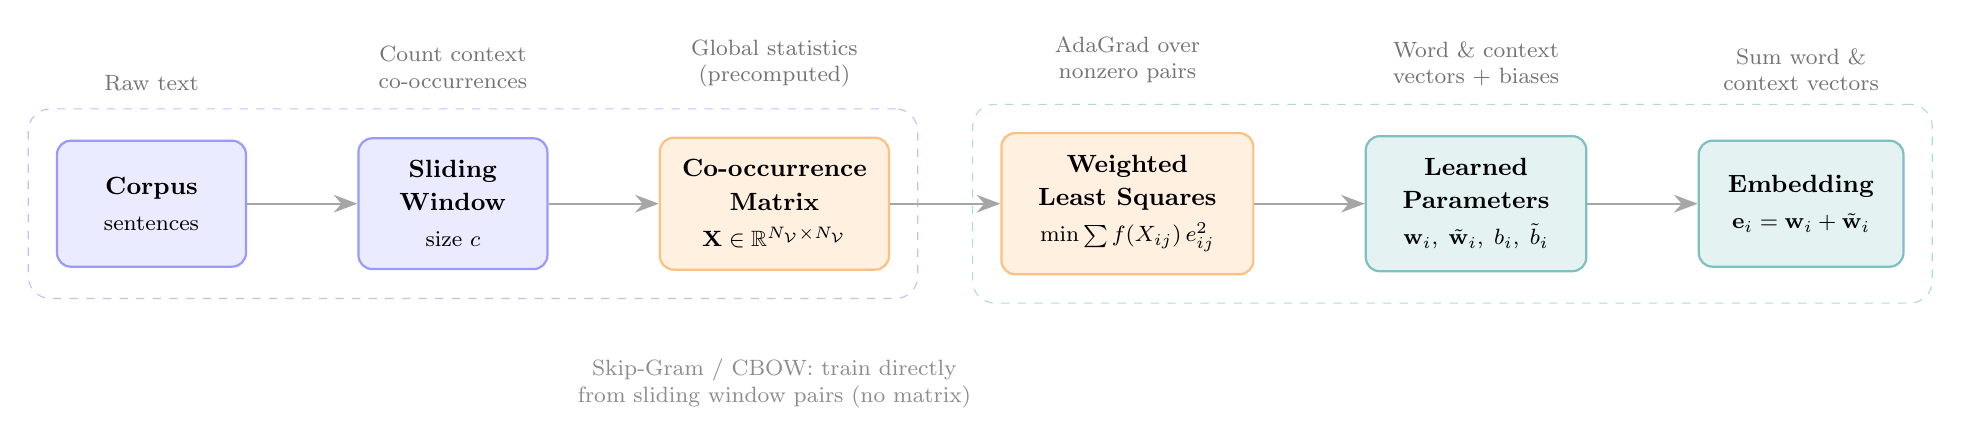
\begin{tikzpicture}[
    stage/.style = {rectangle, draw=gray!60, thick, rounded corners=5pt,
                    minimum height=1.6cm, minimum width=2.4cm,
                    font=\small, inner sep=8pt, align=center},
    arr/.style   = {-{Stealth[length=3mm]}, thick, gray!70},
    label/.style = {font=\footnotesize, text=black!55, align=center},
]

%% ---- Stage 1: Corpus ----
\node[stage, fill=blue!8, draw=blue!40] (corpus) at (0, 0)
    {\textbf{Corpus}\\[2pt]
     {\footnotesize sentences}};

%% ---- Stage 2: Sliding Window ----
\node[stage, fill=blue!8, draw=blue!40, right=1.4cm of corpus] (window)
    {\textbf{Sliding}\\[1pt]\textbf{Window}\\[2pt]
     {\footnotesize size $c$}};

%% ---- Stage 3: Co-occurrence Matrix ----
\node[stage, fill=orange!12, draw=orange!50, right=1.4cm of window,
      minimum width=2.8cm] (matrix)
    {\textbf{Co-occurrence}\\[1pt]\textbf{Matrix}\\[2pt]
     {\footnotesize $\mathbf{X}\in\mathbb{R}^{N_{\mathcal{V}}\times N_{\mathcal{V}}}$}};

%% ---- Stage 4: Weighted Least Squares ----
\node[stage, fill=orange!12, draw=orange!50, right=1.4cm of matrix,
      minimum width=3.2cm] (wls)
    {\textbf{Weighted}\\[1pt]\textbf{Least Squares}\\[2pt]
     {\footnotesize $\min\sum f(X_{ij})\,e_{ij}^{2}$}};

%% ---- Stage 5: Learned Parameters ----
\node[stage, fill=teal!10, draw=teal!50, right=1.4cm of wls,
      minimum width=2.8cm] (params)
    {\textbf{Learned}\\[1pt]\textbf{Parameters}\\[2pt]
     {\footnotesize $\mathbf{w}_{i},\;\tilde{\mathbf{w}}_{i},\;b_{i},\;\tilde{b}_{i}$}};

%% ---- Stage 6: Final Embedding ----
\node[stage, fill=teal!10, draw=teal!50, right=1.4cm of params,
      minimum width=2.6cm] (embed)
    {\textbf{Embedding}\\[2pt]
     {\footnotesize $\mathbf{e}_{i} = \mathbf{w}_{i} + \tilde{\mathbf{w}}_{i}$}};

%% ---- Arrows ----
\draw[arr] (corpus)  -- (window);
\draw[arr] (window)  -- (matrix);
\draw[arr] (matrix)  -- (wls);
\draw[arr] (wls)     -- (params);
\draw[arr] (params)  -- (embed);

%% ---- Top annotations ----
\node[label, above=0.5cm of corpus]
    {Raw text};
\node[label, above=0.5cm of window]
    {Count context\\co-occurrences};
\node[label, above=0.5cm of matrix]
    {Global statistics\\(precomputed)};
\node[label, above=0.5cm of wls]
    {AdaGrad over\\nonzero pairs};
\node[label, above=0.5cm of params]
    {Word \& context\\vectors + biases};
\node[label, above=0.5cm of embed]
    {Sum word \&\\context vectors};

%% ---- Bottom: contrast with Skip-Gram ----
\node[font=\footnotesize, text=black!45, align=center, below=1.0cm of matrix]
    {Skip-Gram / CBOW: train directly\\from sliding window pairs (no matrix)};

%% ---- Bracket grouping count-based vs. optimization ----
\begin{scope}[on background layer]
    \node[draw=blue!25, dashed, rounded corners=8pt, inner sep=10pt,
          fit=(corpus)(window)(matrix),
          label={[font=\scriptsize\bfseries, blue!40]below:Count-Based Stage}] {};
    \node[draw=teal!30, dashed, rounded corners=8pt, inner sep=10pt,
          fit=(wls)(params)(embed),
          label={[font=\scriptsize\bfseries, teal!45]below:Optimization Stage}] {};
\end{scope}

\end{tikzpicture}
\end{document}
